\documentclass[a4paper,10pt]{article}

% Hier die Nummer des Blatts und Autoren angeben.
\newcommand{\blatt}{11}
\newcommand{\autor}{Merlin Steuer, Till Schander, Lennart Bergmann}

\usepackage{hci}

\begin{document}
% Seitenkopf mit Informationen
\kopf
\renewcommand{\figurename}{Figure}

\aufgabe{16}

\subsection{Analyse}
blabla

\subsection{Design}
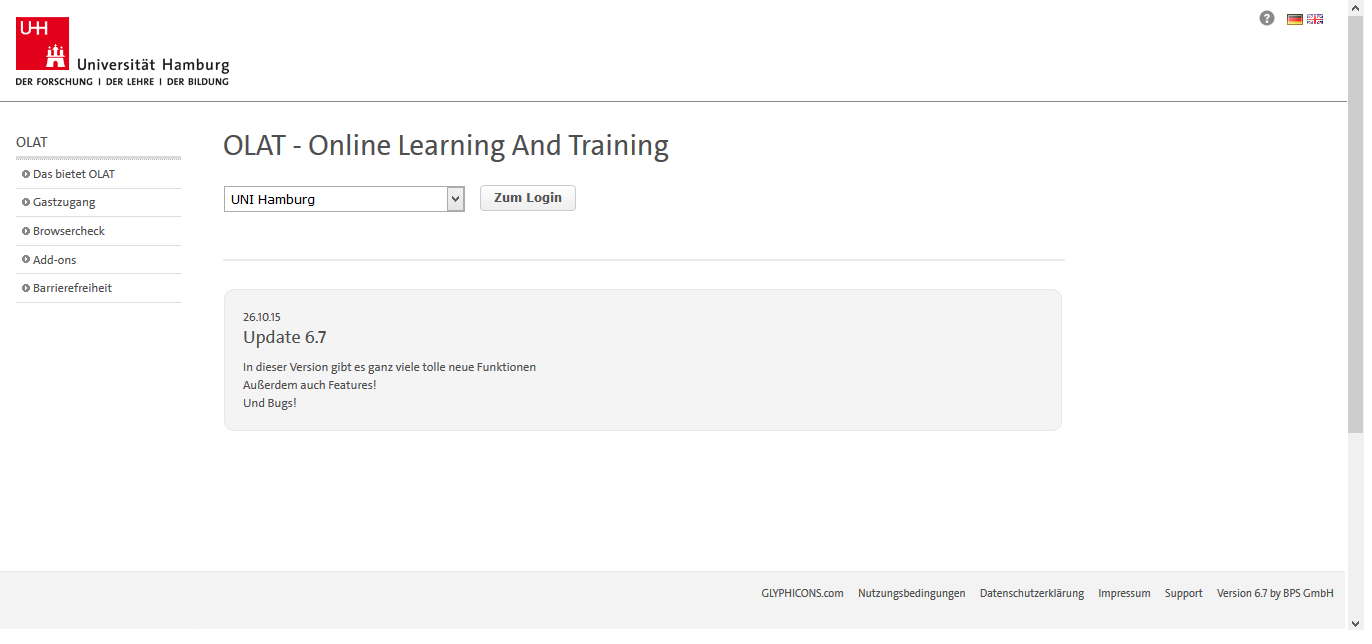
\includegraphics[scale=0.4]{images/login_seite.png}

Die Start-/Login-Seite wurde etwas entschlackt. Die Support-Emails kann man nun unter der Hilfe finden(Merging similiar options). Die Flaggen zur Sprachauswahl sind nun sofort beide sichtbar(exposing options), da ein Dropdown für zwei Optionen überflüssig ist. Das Hauptaugenmerk liegt auf dem Login, da die meisten User dafür die Seite besuchen.

Zudem haben wir uns entschieden den restlichen Platz für einen Newsstream zu nutzen, in dem wichtige Updates oder neue Features angekündigt werden können.


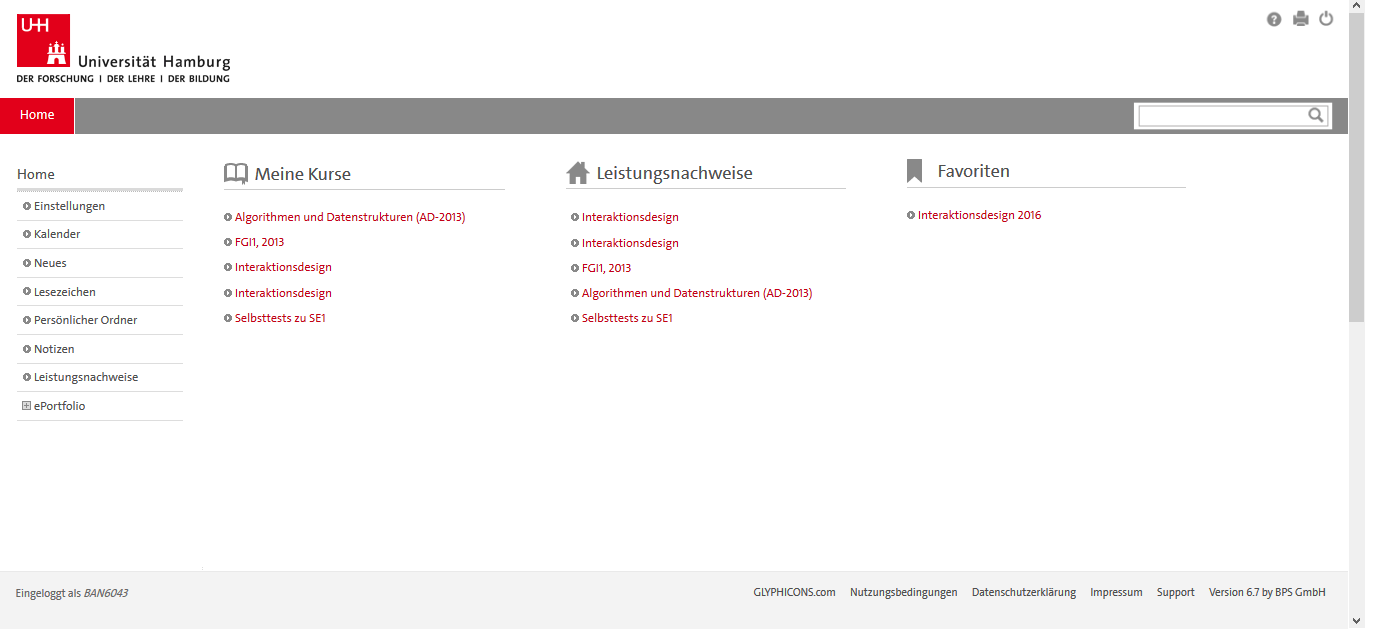
\includegraphics[scale=0.4]{images/wilkommen_seite.png}

Die Wilkommen-Seite wirkte sehr überladen. Wir haben sie etwas aufgeräumt und uns beim re-design auf die wichtigsten Aspekte beschränkt, auch wenn das Dashboard erhalten bleibt. Die meisten User werden OLAT aufrufen um in ihre Kurse zu gucken, oder ihre Bewertungen einzusehen, weshalb wir hierfür einen "Clear Entry Point" geschaffen haben. Die Zeile für "Many Workspaces" bleibt natürlich erhalten, wird aber nur noch für geöffnete Kurse benutzt. Das Hauptaugenmerk liegt darauf, dem Nutzer einen simplere, eingängigere Oberfläche zu präsentieren.

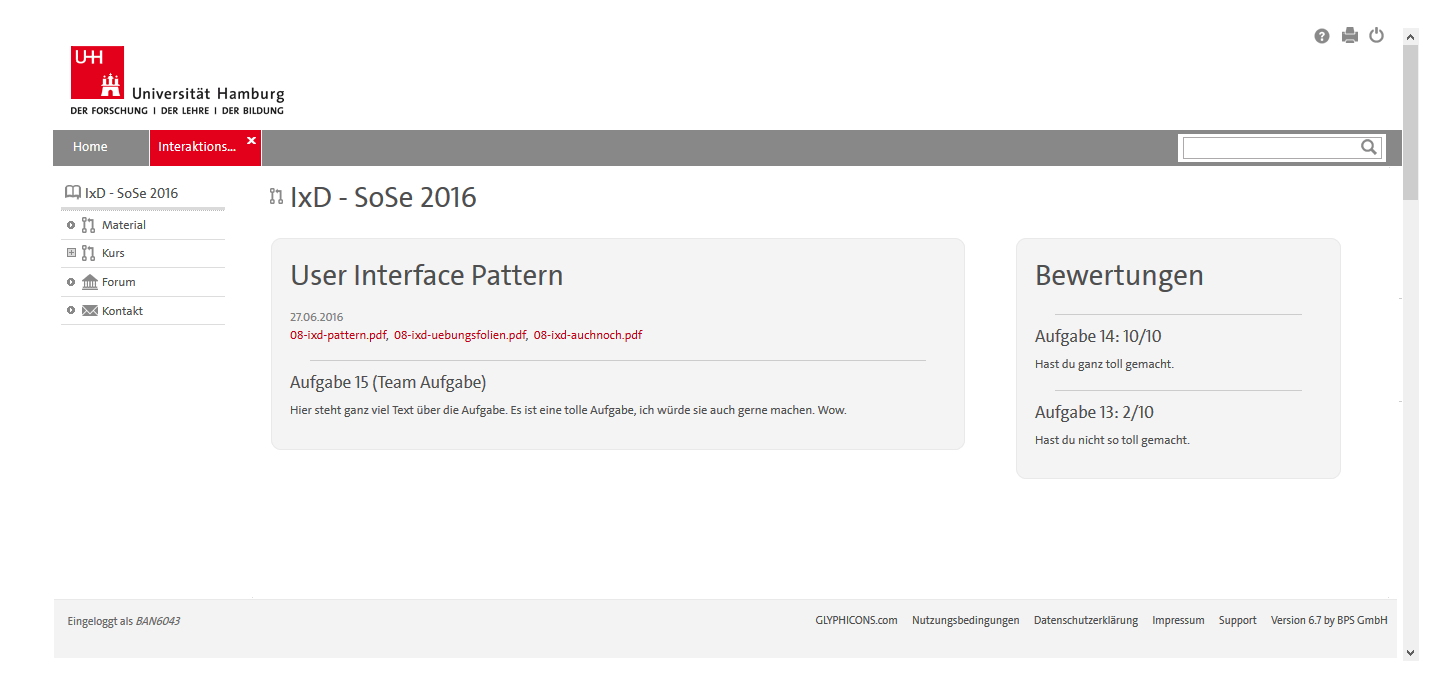
\includegraphics[scale=0.4]{images/ixd_seite.png}

Auch hier haben wir etwas aufgeräumt. Es gibt nun schon auf der Startseite einen Überblick über die neusten Inhalte (Newsstream) sowie die letzten Bewertungen, da die meisten User diese Dinge am ehesten sehen wollen. Die bekannten Seiten bleiben natürlich erhalten(Alternative Views). Der "Ordner" heißt jetzt "Material", damit der User weiß, was ihn hier erwartet. Auch wurden das Wiki, die Linkliste und das Literaturverzeichnis hierhin verschoben, um das Menü zu vereinfachen und zusammengehörige Optionen zu gruppieren. Zur besseren Verständichkeit heißt "Inhalt" jetzt "Kursinhalt" und "Email" wurde zu "Kontakt". Feature/Search/Browse.

Alle Bereiche haben oben links den Escape Hatch, und teilweise zusätzlich noch den Home-Button. 

\subsection{Implementierung} 




\end{document}
